\chapter{Detalles de implementación y experimentos}\label{chapter:implementation}

Para la implementación del modelo y con el objetivo de lograr mejor precisión y generalización, se llevaron a cabo varios experimentos. La metodología de los experimentos fue la misma. Dado que el conjunto de datos utilizado para la validación del modelo está desbalanceado la cantidad de imágenes por clase, en los distintos experimentos se modificó la distribución de datos para aprendizaje, test y validación. Se exponen durante el capítulo 2 de los experimentos que mostraron tener mejores resultados en cuanto a precisión y recobrado. 

\section{Herramientas y Tecnologías}

La implementación del modelo se llevará a cabo utilizando las siguientes herramientas:

\begin{itemize}
    \item \textbf{Lenguajes de Programación:} Python será utilizado por su rica biblioteca de paquetes de aprendizaje automático, incluyendo TensorFlow y Keras para la construcción y entrenamiento del modelo.
    \item \textbf{Frameworks de Aprendizaje Profundo:} TensorFlow y Keras proporcionan las funcionalidades necesarias para diseñar, entrenar y validar modelos de aprendizaje profundo con alta eficiencia y flexibilidad.
    \item \textbf{Técnicas de Preprocesamiento:} Herramientas para la normalización de imágenes, el aumento de datos, y el balanceo de clases serán utilizadas para preparar el dataset para el entrenamiento del modelo.
    \item \textbf{Optimización y Regularización:} Se integrarán técnicas como el ajuste dinámico del learning rate y la regularización L1 y L2 para optimizar el rendimiento del modelo y prevenir el sobre-ajuste.
    \item \textbf{Hardware y Recursos Computacionales:} Se utilizó Google Collab para acelerar el proceso de entrenamiento del modelo, permitiendo la experimentación con diferentes híper-parámetros y arquitecturas de forma eficiente.
\end{itemize}

\section{Enfoque de Implementación}

La implementación seguirá un enfoque modular y escalable. Comenzará con la selección del modelo y su personalización para el contexto específico del cáncer de piel. El preprocesamiento de datos y el balanceo de clases asegurarán la calidad del entrenamiento y la generalización del modelo. La arquitectura del modelo será iterativamente refinada y evaluada, utilizando un algoritmo propio de ajuste de precisión Además se utilizan capas adicionales de ajuste y optimización para lograr mejores resultados.
\section{Dataset}

El dataset utilizado como medio de aprendizaje para este proyecto es HAM1000-segmentation-and-classification \brackcite{ham10000}. Este conjunto de datos, acrónimo de Human Against Machine (Humano contra máquina) con 10000 imágenes de entrenamiento, es una amplia colección de imágenes dermatoscópicas. En concreto, contiene 10015 imágenes del archivo ISIC, que inicialmente formaban parte de un conjunto de entrenamiento creado por ISIC \brackcite{tschandl2018ham10000} con la siguiente distribución.


\begin{tabular}{lrr}
   \hline
   \textbf{Categoría Diagnóstica} & \textbf{Número de Imágenes} & \textbf{Porcentaje} \\
   \hline
   Melanocytic nevi               & 6705                        & 66.95\%             \\
   Melanoma                       & 1113                        & 11.11\%             \\
   Benign keratosis-like lesions  & 1099                        & 10.97\%             \\
   Basal cell carcinoma           & 514                         & 5.13\%              \\
   Actinic keratoses              & 327                         & 3.27\%              \\
   Vascular lesions               & 142                         & 1.42\%              \\
   Dermatofibroma                 & 115                         & 1.15\%              \\
   \hline
   \end{tabular}

\section{Preparación y carga de datos}

Los datos utilizados como medio de aprendizaje para este proyecto son imágenes y metadatos. El dataset HAM10000 contiene imágenes tomadas de varios tipos de cáncer de piel y un archivo de metadatos que contienen información relacionada con cada imagen en formato \textit{one hot encoding}. Esta una técnica de procesamiento de datos en la cual cada valor categórico se representa mediante un vector binario cuyo tamaño corresponde al número de categorías posibles. En dicho vector, todos los elementos son cero, salvo el correspondiente a la categoría del valor, que es uno \brackcite{ohe}.

\subsection{Transformación de datos}

Para optimizar la eficiencia del algoritmo, se procesan las imágenes realizando diversas modificaciones, que incluyen: eliminación de cabello, luces y sombras, división de canales y aplicación de un leve desenfoque.

Los metadatos asociados a la clasificación, etiquetados con método mencionado, fueron convertidos a un formato \textit{categórico} \brackcite{vitalflux_categorical_crossentropy} para su procesamiento. Se define \textit{categórico} como el formato en el que a cada elemento se le asigna el nombre de una categoría como propiedad.

\subsection{Modelación y división del conjunto de datos}

Los datos se modelan a partir de un dataframe de Pandas \brackcite{pandas}. Estos son divididos en 3 conjuntos: Entrenamiento, Validación y Prueba, utilizando un enfoque simple de division de datos en porcentaje. Estas divisiones son necesarias para que el modelo pueda aprender y ser evaluado correctamente.

Inicialmente, el conjunto de datos, fue dividido en dos subconjuntos: \textit{train}, que se destinó para el entrenamiento, y \textit{dummy}, que fue utilizado como una combinación temporal para los conjuntos de validación y prueba. Luego el segundo conjunto fue separado en \textit{valid}, destinado a la validación y \textit{test}, utilizado para las pruebas.

\subsubsection{Experimento 1}

   La distribución de datos fue la siguiente:

   \begin{enumerate}
      \item El 95\% de los datos se destinan al conjunto de entrenamiento.
      \item El 2.5\% de los datos restantes se destinan al conjunto de validación.
      \item El 2.5\% restante se destina al conjunto de pruebas.
   \end{enumerate}
   
   Además se mezclan aleatoriamente los datos y se utiliza una variable fija para garantizar que la división sea reproducible. Aquí se utiliza \textit{dummy split} para mantener la proporción deseada entre validación y prueba. Por lo que este experimento tiene $9514$ datos de entrenamiento, $251$ de test y $250$ de validación.

   \begin{table}[ht]
      \centering
      \begin{tabular}{lccc}
      \hline
      \textbf{Diagnostic category} & \textbf{Training} & \textbf{Validation} & \textbf{Testing} \\
      \hline
      NV       & 300 & 158 & 163 \\
      MEL      & 300 & 25  & 35  \\
      BKL      & 300 & 34  & 30  \\
      DF       & 115 & 5   & 3   \\
      AKIEC    & 300 & 11  & 7   \\
      BCC      & 300 & 16  & 10  \\
      VASC     & 142 & 1   & 3   \\ \hline
      \end{tabular}
      \caption{Experimento 1: Distribución de imágenes de cáncer de piel en los conjuntos de entrenamiento, test y validación}
      \label{table:train_test_validate_e1}
      \end{table}
   



\subsubsection{Experimento 2}

La distribución de datos fue la siguiente:

   \begin{enumerate}
      \item El 70\% de los datos se destinan al conjunto de entrenamiento.
      \item El 15\% de los datos restantes se destinan al conjunto de validación.
      \item El 15\% restante se destina al conjunto de pruebas.
   \end{enumerate}
   
Se utiliza \textit{stratify} en ambas divisiones para mantener la distribución de etiquetas \textit{label} en cada conjunto. Se calcula la proporción del conjunto de prueba sobre la suma del conjunto de test y el de validación.

   \begin{table}[ht]
      \centering
      \begin{tabular}{lccc}
      \hline
      \textbf{Diagnostic category} & \textbf{Training} & \textbf{Validation} & \textbf{Testing} \\
      \hline
      NV    & 300 & 1006 & 1006 \\
      MEL   & 300 & 167  & 167  \\
      BKL   & 300 & 165  & 165  \\
      DF    & 300 & 17   & 17   \\
      AKIEC & 300 & 49   & 49   \\
      BCC   & 300 & 77   & 77   \\
      VASC  & 300 & 21   & 22   \\
      \hline
      \end{tabular}
      \caption{Experimento 2: Distribución de imágenes de cáncer de piel en los conjuntos de entrenamiento, test y validación}
      \label{tab:train_test_validate_e2}
      \end{table}
      

Luego este quedaría distribuido en $7010$ datos de entrenamiento, $1503$ de test y $1502$ de validación.

\section{Generadores de datos y preprocesamiento}

Uno de los principales problemas del dataset, es el desequilibrio en la representación de las clases, un problema habitual en los conjuntos de datos médicos en los que algunas enfermedades son más raras que otras. Para solucionar este problema, el conjunto de datos se equilibra meticulosamente limitando el número máximo de muestras por clase ($300$). Esto garantiza que el modelo no esté sesgado hacia las clases más comunes y pueda generalizar mejor entre varios tipos de lesiones cutáneas.

\subsection{Experimento 1}

Se establece para este un tamaño objetivo de muestras por clase ($300$ en este caso), y se utiliza un bucle para iterar a través de cada clase única. Se realiza un re-muestreo con reemplazo para clases con un número de muestras menor al objetivo ($300$), y sin reemplazo para clases con un número igual o mayor al tamaño objetivo.

\begin{table}[ht]
   \centering
   \begin{tabular}{lccc}
   \hline
   Diagnostic category & Sampling  \\ \hline
   AKIEC & 300 \\
   BCC & 300 \\
   BKL & 300 \\
   DF & 115 \\
   MEL & 300 \\
   NV & 300 \\
   VASC & 142 \\ \hline
   \end{tabular}
   \caption{Distribución de muestras por categoría después del sobre-muestreo}
   \label{tab:sampling_distribution_1}
   \end{table}


Como se evidencia anteriormente, al separar la data en clases el conjunto se mantiene desbalanceado. Se hace necesario aplicar un método llamado \textit{Class Weighting} \brackcite{analyticsvidhya2020classweight}. Este método se refiere a la asignación de pesos diferenciados a cada clase durante el proceso de entrenamiento del modelo, con el objetivo de reforzar la señal de entrenamiento de las clases menos representadas, o sea, las clases/categorías con menos cantidad de datos:

\begin{table}[ht]
   \centering
   \begin{tabular}{lccc}
   \hline
   Diagnostic category & Sampling  & Weighting\\ \hline
   AKIEC & 300 & 1.00\\
   BCC & 300 & 1.00\\
   BKL & 300 & 1.00\\
   DF & 115 & 2.60\\
   MEL & 300 & 1.00\\
   NV & 300 & 1.00\\
   VASC & 142 & 2.11\\ \hline
   \end{tabular}
   \caption{Distribución de muestras con peso asignado}
   \label{tab:weighting_distribution}
   \end{table}

\subsection{Experimento 2}

Se establece también un tamaño objetivo de muestras por clase ($300$). Se utiliza la función \textit{groupby} para agrupar el dataFrame por la etiqueta de clase. Se itera sobre cada grupo, y se realiza un re-muestreo con reemplazo para grupos menores al tamaño deseado y sin reemplazo para los grupos que ya alcanzan o superan el tamaño deseado.

En este, a diferencia del primero, en cada clase se alcanza la misma cantidad de muestras, por lo que no es necesario aplicar \textit{Class Weighting}.

\begin{table}[ht]
   \centering
   \begin{tabular}{lccc}
   \hline
   Diagnostic category & Sampling  \\ \hline
   AKIEC & 300 \\
   BCC & 300 \\
   BKL & 300 \\
   DF & 300 \\
   MEL & 300 \\
   NV & 300 \\
   VASC & 300 \\ \hline
   \end{tabular}
   \caption{Distribución de muestras por categoría después del sobre-muestreo}
   \label{tab:sampling_distribution}
   \end{table}

\subsection{Aumento y división de datos}

Para la carga y procesamiento de imágenes se utilizó la clase ImageDataGenerator de Keras \brackcite{img_gen}. Esta clase es una parte integral de la biblioteca Keras y proporciona una forma eficiente de manipular imágenes para tareas de aprendizaje automático. Su principal función es facilitar la creación de lotes de imágenes que se utilizan durante el entrenamiento y la evaluación de modelos de Machine Learning, especialmente en el contexto de redes neuronales. 

Se inicializa con varias transformaciones (como rotación, desplazamiento y zoom) aplicadas automáticamente a las imágenes a medida que se cargan, para devolver lotes de imágenes listos para el entrenamiento o la evaluación del modelo \brackcite{augmentation}.

\begin{table}[ht]
   \centering
   \begin{tabular}{lccc}
   \hline
   Parámetro & Descripción  & Valor \\ \hline
   rotation range & 	Rango de rotación & 20 grados \\
   width shift range & Rango de desplazamiento horizontal & 20\% \\
   height shift range & Rango de desplazamiento vertical & 20\% \\
   shear range & 	Rango de corte & 20\% \\
   zoom range & Rango de zoom & 20\% \\
   horizontal flip & Activación de volteo horizontal & verdadero \\
   fill mode & Modo de relleno para manejar los píxeles faltantes & nearest \\ \hline
   \end{tabular}
   \caption{Parámetros de aumento de datos}
   \label{tab:data_augmentation_params}
   \end{table}

\section{Diseño y entrenamiento del modelo}

Se utiliza la arquitectura de red neural denominada \textit{EfficientNetB1} \brackcite{efficientnet}. Esta arquitectura forma parte de la familia EfficientNet, que está diseñada para proporcionar alta precisión mientras se mantiene un tamaño de modelo y una complejidad computacional eficientes.

Para aprovechar los conocimientos previos y acelerar el entrenamiento, se carga el modelo \textit{EfficientNetB1} pre-entrenado con los pesos obtenidos al procesar el dataset \textit{ImageNet}. El mismo consiste en una amplia base de datos de imágenes utilizada comúnmente para entrenamiento y \textit{benchmarking} en tareas de visión por computadora. Utilizar este modelo pre-entrenado permite aprovechar las características que ya ha aprendido de este amplio conjunto de datos, facilitando su adaptación al dataset HAM10000.

Se utiliza el \textit{EfficientNetB1} sin incluir su capa superior, con el objetivo de añadir y personalizar capas adicionales. Tras obtener la salida del modelo base, se aplica una serie de transformaciones, incluyendo normalización por lotes, una capa densa con regularizaciones, una técnica de \textit{Dropout} para prevenir el sobre-ajuste y una capa de optimización. 

\subsection{ImageNet}

ImageNet es un proyecto de base de datos visual extenso, diseñado principalmente para la investigación en reconocimiento visual de objetos. Contiene más de 14 millones de imágenes, anotadas manualmente para indicar qué objetos se muestran, y más de 20,000 categorías, cada una con cientos o miles de imágenes. Este proyecto ha sido fundamental en el avance de la visión por computadora y el aprendizaje profundo, proporcionando un recurso de datos inmenso y diverso para entrenar algoritmos de inteligencia artificial.

La relevancia de ImageNet para el aprendizaje profundo se puso de manifiesto con el éxito de AlexNet en el desafío ImageNet 2012 \brackcite{Pinecone2021ImageNet}, donde logró una tasa de error top-5 del 15.3\%, notablemente inferior a la de sus competidores. Este hito marcó un punto de inflexión en el campo, demostrando la viabilidad y la potencia de las redes neuronales convolucionales (CNN) cuando se combinan con unidades de procesamiento gráfico (GPU) para el entrenamiento.

\subsection{Arquitectura del modelo EfficientNet}

La familia de arquitecturas EfficientNet, desarrollada por los autores en \brackcite{tan2019efficientnet}, surgió con el objetivo de hallar un método adecuado para escalar las CNNs de manera que mejoraran tanto en precisión (i.e., rendimiento del modelo) como en eficiencia (es decir, en términos de parámetros del modelo y FLOPS). Estos autores propusieron un método de escalado compuesto que utiliza un conjunto fijo de coeficientes para escalar de manera uniforme el ancho, la profundidad y la resolución de la red. El método les permitió desarrollar una arquitectura de CNN eficiente, a la que denominaron EfficientNet B0. Posteriormente, crearon las variantes EfficientNets B1-B7 escalando la red base (EfficientNet B0).

Mientras que la arquitectura EfficientNet B0 tiene $5.3$ millones de parámetros y acepta imágenes de entrada de $224x224$, EfficientNet B7 cuenta con $66$ millones de parámetros y acepta imágenes de $600x600$ \brackcite{Tan2019EfficientNetRM}.

\begin{figure}[ht]%
   \begin{center}
   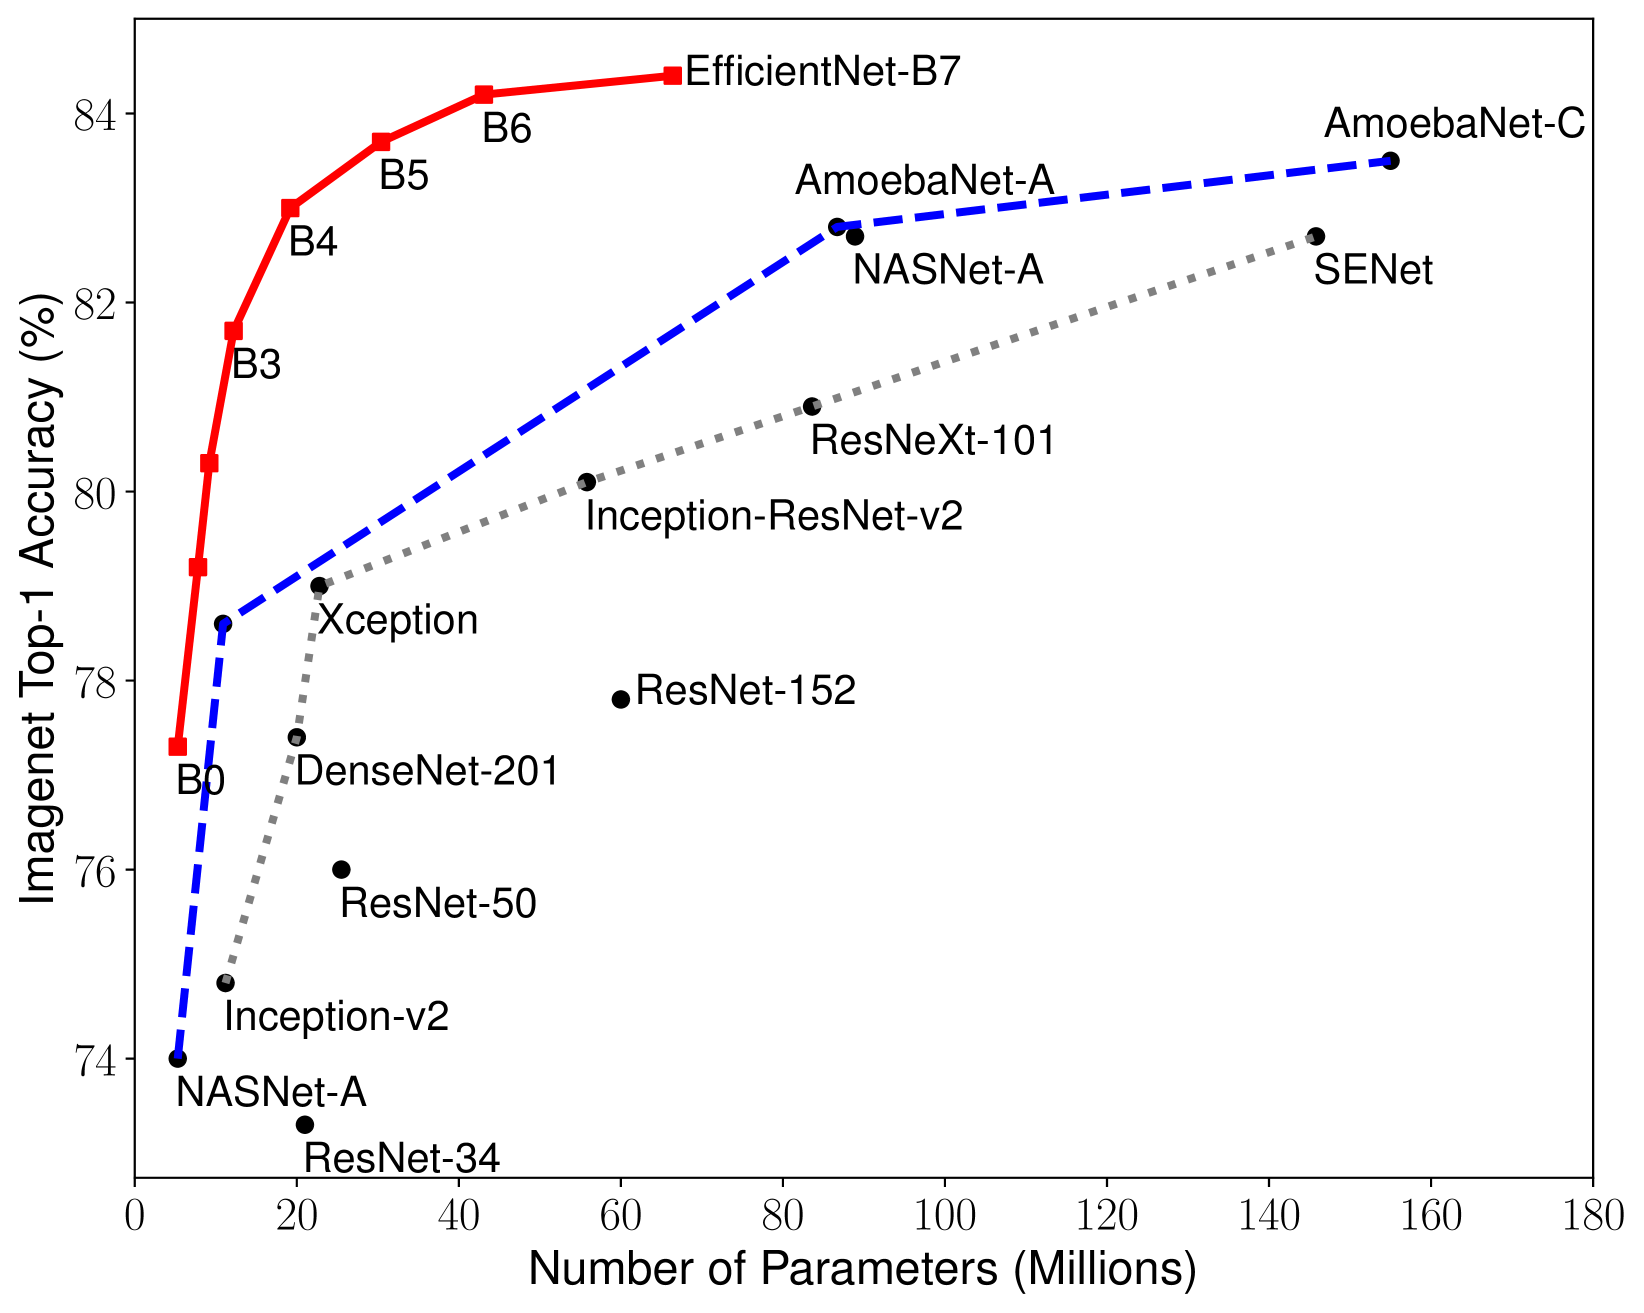
\includegraphics[width=1\textwidth]{./Graphics/efficientnet_performance.png}
   \caption{Estadísticas del rendimiento de los modelos de EfficientNet}
   \label{fig:efficientnet_performance}
   \end{center}
   \end{figure}

\subsection{EfficientNetB1}

En relación con el dataset HAM1000 \brackcite{ham10000}, la implementación del EfficientNetB1 puede ser particularmente beneficiosa para el análisis de datos. EfficientNetB1, entre las variantes de la serie EfficientNet, se encuentra en un punto medio en términos de complejidad y tamaño, ofreciendo un equilibrio entre precisión y eficiencia computacional. Dado que el HAM1000 es un conjunto de datos de imágenes dermatoscópicas que requiere una alta precisión en la identificación y clasificación de lesiones cutáneas, la utilización de EfficientNetB5 podría proporcionar una precisión y eficiencia aceptable en términos de recursos computacionales.

\subsection{Capas adicionales y regularización}

Para ajustar el modelo de EfficientNetB1 a nuestras necesidades, se añaden capas adicionales:

\subsubsection{Normalización por lotes}

Para mejorar la estabilidad y eficiencia del modelo EfficientNetB1, se incorpora una capa de Normalización por lotes. La normalización por lotes es crucial para estabilizar las \textit{activaciones} a lo largo de las capas del modelo. Al estandarizar las activaciones por lote, mejora la eficiencia del entrenamiento y permite el uso de tasas de aprendizaje más altas. Esta técnica contribuye significativamente a la regularización del modelo, reduciendo el riesgo de sobre-ajuste y facilitando un aprendizaje más rápido y estable.

Esta capa se define con un \textit{eje de normalización} establecido en $-1$, lo que indica que la normalización se aplica a lo largo del último eje en el tensor de entrada. Además, se configura un \textit{momentum} de $0.99$ y un valor de \textit{epsilon} de $0.001$. El alto valor de momentum ayuda a mantener la estabilidad de las medias y varianzas móviles a lo largo del entrenamiento, mientras que el pequeño valor de epsilon evita divisiones por cero, asegurando así cálculos numéricos estables \brackcite{regularization}.

\subsubsection{Capa densa}

Se integra una capa densa con $256$ neuronas, que juega un papel clave en la síntesis de las características aprendidas por el modelo. Se utiliza un regularizador \textit{L2} con un \textit{lambda} de $0.016$ para los pesos de la capa, lo que ayuda a penalizar y controlar el tamaño de los pesos, reduciendo así el riesgo de sobre-ajuste. Además, tanto el regularizador de actividad como el regularizador de bias se configuran con un regularizador \textit{L1} con un \textit{lambda} de $0.006$. Este enfoque impone una penalización en los pesos y los sesgos, promoviendo un modelo más simple y disperso. La función de activación utilizada es \textit{ReLU} , conocida por su eficacia en la introducción de no linealidad en el modelo, lo que permite aprender relaciones complejas entre las características \brackcite{dense}.

\subsubsection{Dropout}

En la arquitectura del modelo, se integra una capa de dropout para aumentar la robustez y prevenir el sobre-ajuste. Esta capa se configura con una tasa de desactivación del 45\% , lo que significa que, durante el entrenamiento, el 45\% de las neuronas se desactivarán aleatoriamente en cada paso. 

En una primera iteración del algoritmo tuvo una tasa de desactivación más baja. Luego de varias iteraciones se concluyó que se necesitaba un algoritmo de clasificación que estudiara más a detalle la data fomentando así una mejor generalización y reduciendo el riesgo de sobre-ajuste en el proceso de aprendizaje. Basándonos en esto aumentamos la tasa y obtuvimos mejores resultados.

Para asegurar la reproducibilidad, se establece una semilla(seed) $123$. Esta introducción de aleatoriedad ayuda a que el modelo no dependa excesivamente de ninguna característica o neurona específica \brackcite{dropout}.

\subsubsection{Capa de salida}

La capa de salida utiliza una activación \textit{softmax} para transformar las salidas del modelo en probabilidades de pertenencia a cada clase. Esto, clasifica las entradas en categorías distintas, proporcionando probabilidades para cada clase, lo cual es esencial en la clasificación multi-clase.

\subsection{Optimización}

Para el proceso de entrenamiento, se utiliza el optimizador \textit{Adamax} \brackcite{adamax}. Este es una variante del conocido optimizador Adam, que combina las ventajas de los métodos adaptativos de tasa de aprendizaje con una implementación más robusta en entornos con gradientes dispersos, lo cual es común en imágenes médicas 

La función de pérdida elegida es la \textit{categorical crossentropy} \brackcite{vitalflux_categorical_crossentropy}, idónea para problemas de clasificación multi-clase. Se configura el modelo para minimizarla y se rastrea la precisión como métrica principal.

\subsection{Ajuste dinámico de la tasa de aprendizaje}

Un componente innovador de nuestro enfoque es el uso de un Callback personalizado para el ajuste dinámico del learning rate \brackcite{lr}, basado en la precisión del entrenamiento y la pérdida de validación. Este mecanismo adapta el learning rate durante el entrenamiento, reduciéndolo si el modelo no mejora a un ritmo esperado. Este ajuste es vital en la navegación de superficies de pérdida complejas, aumentando la probabilidad de que el modelo evite mínimos locales subóptimos y converja hacia soluciones más efectivas.

%-----------------------------------------------------------------------------------
\section{Resultados}\label{sec:results}
%-----------------------------------------------------------------------------------

En esta sección presentamos los resultados obtenidos. Nuestro enfoque se centró en la exploración y optimización de dos pipelines de procesamiento y clasificación de imágenes. Los experimentos se estructuraron con el objetivo de evaluar mejoras de precisión en el modelo utilizando distintas aproximaciones de procesamiento y normalización de datos y optimizadores en el contexto del procesamiento de imágenes.

Tras la implementación del modelo, los resultados obtenidos superan las espectativas. El modelo con mayor eficiencia luego de varios ajustes tuvo una eficacia de validación cercana al 84\%. Los resultados son un paso significativo hacia la automatización del diagnóstico del cáncer de piel, que tradicionalmente ha dependido de la inspección visual por parte de expertos humanos. 

En cada sección se muestran algunas métricas que muestran el desarrollo del modelo, con los siguientes parámetros:

\begin{table}[ht]
   \centering
   \small
   \begin{tabular}{|c|p{10cm}|}
   \hline
   \textbf{Término} & \textbf{Descripción} \\
   \hline
   Epoch & Es una iteración completa sobre todo el conjunto de datos de entrenamiento. \\
   \hline
   Loss (Pérdida) & Es una medida de cuán bien el modelo está realizando sus predicciones. Los valores decrecientes indican una mejora en el aprendizaje. \\
   \hline
   Accuracy (Precisión) & Muestra el porcentaje de etiquetas que el modelo predice correctamente para el conjunto de entrenamiento. \\
   \hline
   V loss (Pérdida de Validación) & Es similar a la pérdida, pero se calcula sobre un conjunto de datos que no se utiliza para el entrenamiento. \\
   \hline
   V acc (Precisión de Validación) & Muestra el porcentaje de etiquetas que el modelo predice correctamente para el conjunto de datos de validación. \\
   \hline
   LR (Learning Rate) & La tasa de aprendizaje dicta cuánto se ajustan los pesos del modelo en cada actualización. \\
   \hline
   Next LR (Próxima Learning Rate) & Indica la próxima tasa de aprendizaje planificada. La adaptación de la tasa de aprendizaje puede ayudar a evitar el estancamiento y mejorar la convergencia. \\
   \hline
   Monitor & Muestra la métrica que se está utilizando para monitorizar el rendimiento del modelo. Cambia de \textit{accuracy} a \textit{val loss}, lo que probablemente indica que el cambio se hizo para evitar el sobre'ajuste. \\
   \hline
   Duration (Duración) & Tiempo que tardó cada epoch en completarse. Importante para evaluar la eficiencia del entrenamiento. \\
   \hline
   \end{tabular}
   \caption{Descripción de términos clave en el entrenamiento de modelos de aprendizaje automático.}
   \label{table:terminology}
   \end{table}
   

\subsection{Experimento 1}

%-----------------------------------------------------------------------------------
	\subsubsection{Estadísticas básicas}\label{sub:basic_statistics_p1}
%-----------------------------------------------------------------------------------
    
    Estos resultados de la tabla siguiente corresponden a la evaluación del modelo a lo largo de 40 epochs (o iteraciones) de entrenamiento.

    \begin{figure}[ht]
      \small
      \begin{center}
          \begin{tabular}{|c|c|c|c|c|c|c|c|} \hline
          E & Loss & Acc & V loss & V acc & LR & M & Batch \\ \hline
          1 & 9.587 & 40.581 & 8.95658 & 56.800 & $10^{-2}$ & accuracy & 85.25 \\ \hline
          2 & 7.798 & 67.615 & 7.67235 & 66.800 & $10^{-2}$ & accuracy & 21.72 \\ \hline
          3 & 6.884 & 79.340 & 6.96014 & 69.600 & $10^{-2}$ & accuracy & 22.56 \\ \hline
          4 & 6.214 & 87.365 & 6.35865 & 71.200 & $10^{-2}$ & accuracy & 25.81 \\ \hline
          5 & 5.646 & 91.690 & 5.94812 & 75.200 & $10^{-2}$ & val\_loss & 23.08 \\ \hline
          6 & 5.172 & 92.999 & 5.44954 & 76.800 & $10^{-2}$ & val\_loss & 23.23 \\ \hline
          7 & 4.735 & 94.479 & 5.06016 & 76.400 & $10^{-2}$ & val\_loss & 23.19 \\ \hline
          8 & 4.334 & 96.528 & 4.73837 & 76.800 & $10^{-2}$ & val\_loss & 22.90 \\ \hline
          9 & 3.969 & 97.211 & 4.33689 & 77.200 & $10^{-2}$ & val\_loss & 22.74 \\ \hline
          10 & 3.631 & 98.008 & 4.15826 & 74.000 & $10^{-2}$ & val\_loss & 22.56 \\ \hline
          11 & 3.315 & 98.406 & 3.89153 & 73.600 & $10^{-2}$ & val\_loss & 23.11 \\ \hline
          \dots & \dots & \dots & \dots & \dots & \dots & \dots & \dots \\ \hline
          34 & 0.627 & 99.886 & 1.24470 & 76.800 & 0.00013 & val\_loss & 23.30 \\ \hline
          \end{tabular}
          \caption{Estadísticas básicas del modelo EfficientNetB1.}
      \end{center}\label{fig:estadisticas_p1}
  \end{figure}
    
  Aquí vemos que el entrenamiento se planeó para 40 epochs, pero se detuvo en el epoch 34, después de tres ajustes de la tasa de aprendizaje sin mejoras en la pérdida de validación. Esto ocurre dado que el modelo no estaba mejorando su capacidad de generalizar a datos no vistos y que continuar el entrenamiento probablemente habría resultado en un gasto innecesario de recursos y posiblemente en un mayor sobre-ajuste. 
  
  En la tabla se observa que la precisión de entrenamiento aumenta con cada epoch, la pérdida de entrenamiento disminuye consistentemente, la tasa de aprendizaje permanece constante al principio y luego disminuye para afinar el entrenamiento a medida que el modelo comienza a converger, todo lo anterior es indicador que el modelo esta entrenando de forma correcta.

  En el monitor se muestra que cambia de \textit{accuracy} a \textit{val loss}, este cambio se hizo para evitar el sobre-ajuste.

%-----------------------------------------------------------------------------------
\subsubsection{Estadísticas de aprendizaje}\label{sub:learning_statistics_p1}
%-----------------------------------------------------------------------------------
		\begin{figure}[ht]%
      \begin{center}
      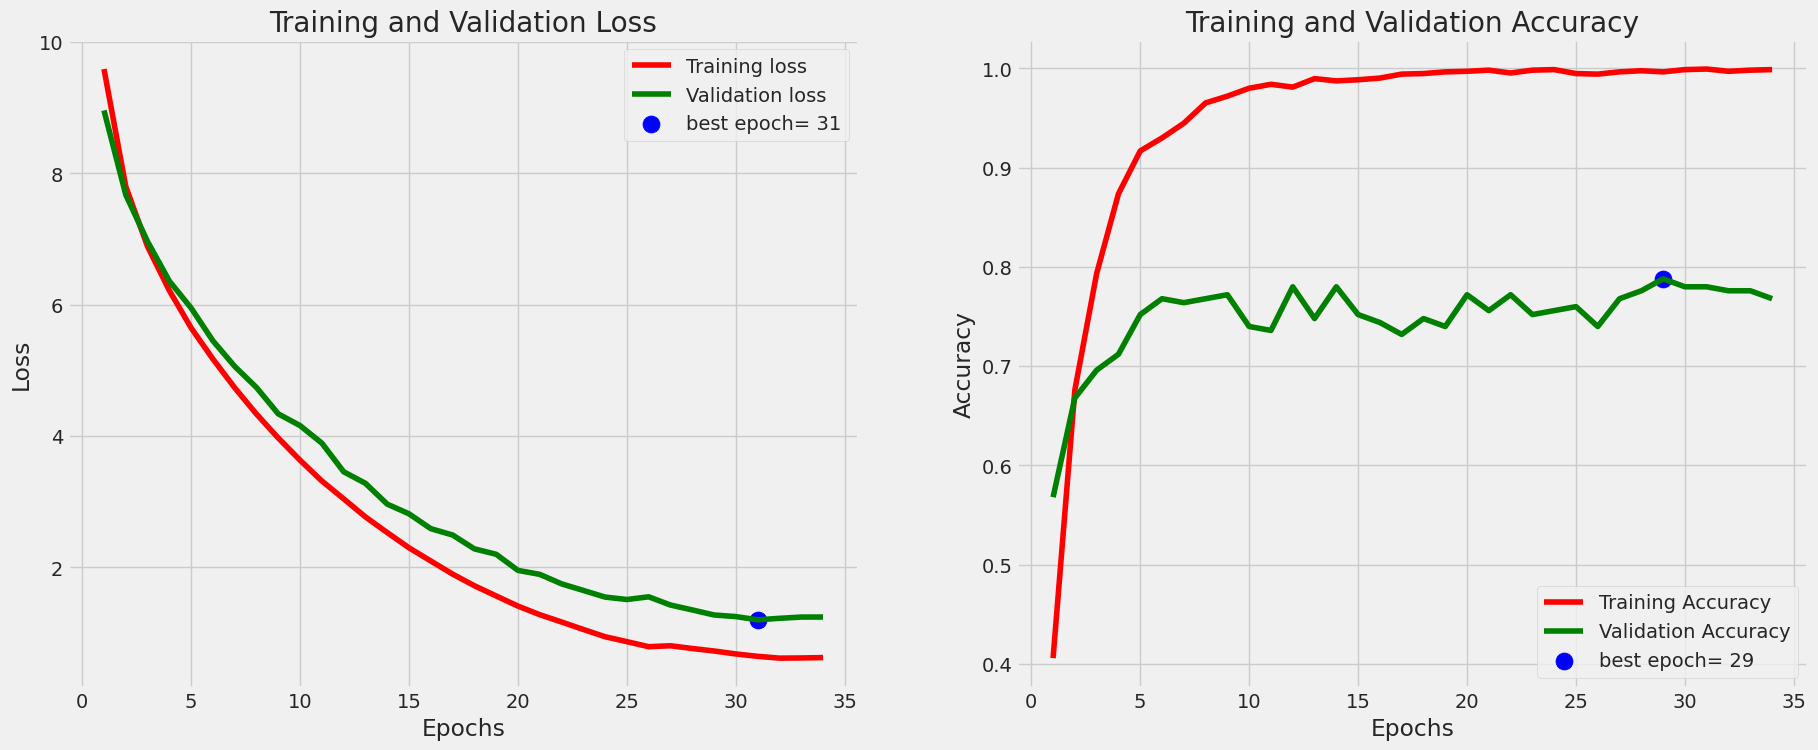
\includegraphics[width=1\textwidth]{./Graphics/training&validation_p1.png}
      \caption{Estadísticas de aprendizaje a lo largo del proceso de entrenamiento.\label{fig:training_validation_loss}}
      \end{center}
		\end{figure}
  
La imagen anterior muestra dos gráficos, uno de pérdida y otro de precisión respectivamente, a lo largo de los epochs de entrenamiento y validación. El primero muestra una disminución constante de la pérdida tanto en el entrenamiento como en la validación, lo cual es indicativo de un buen aprendizaje. La pérdida de validación tiene un mínimo en el epoch 31, lo que sugiere que este podría ser el mejor modelo para evitar el sobre-ajuste. A partir de este punto, si la pérdida de validación comenzase a aumentar mientras la pérdida de entrenamiento sigue disminuyendo, indicaría sobre-ajuste.

En el segundo se aprecia como la precisión de entrenamiento aumenta rápidamente y luego se estabiliza cerca del 100\%, mientras que la precisión de validación también aumenta pero con cierta variabilidad entre los epochs. El mejor epoch según la precisión de validación es el 29. Esta diferencia entre la precisión de entrenamiento y de validación sugiere que puede haber variabilidad en los datos de validación.

%-----------------------------------------------------------------------------------
	\subsubsection{Estadísticas de eficacia}\label{sub:accuracy_statistic_p1}
%-----------------------------------------------------------------------------------
\begin{figure}[ht]%
   \begin{center}
   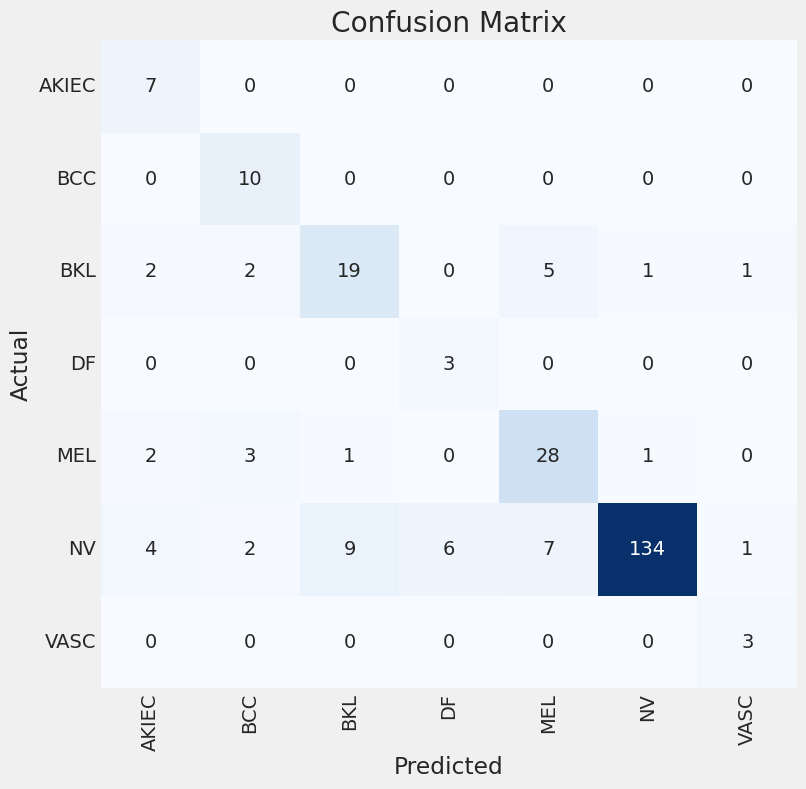
\includegraphics[width=1\textwidth]{./Graphics/confussionmatrix_p1.png}
   \caption{Estadísticas de eficacia del modelo al estimar los resultados en el conjunto de pruebas\label{fig:confussion_matrix_p1}}
   \end{center}
   \end{figure}

   \begin{figure}[ht]%
      \begin{center}
      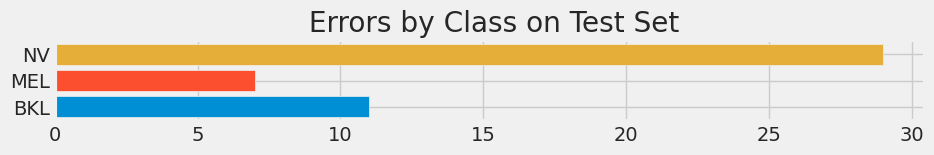
\includegraphics[width=1\textwidth]{./Graphics/errorByClass_p1.png}
      \caption{Gráfico de errores por clase en el conjunto de pruebas\label{fig:class_errors_p1}}
      \end{center}
      \end{figure} 


La matriz de confusión proporciona información valiosa sobre el rendimiento del modelo en relación de Actual/Predicho, en términos de su capacidad para clasificar correctamente cada una de las siete clases de cáncer de piel. La diagonal principal de la matriz representa los verdaderos positivos (TP), el número de casos en los que el modelo ha predicho correctamente la clase correspondiente. Los valores fuera de la diagonal principal indican errores de clasificación.

    La clase 'NV' muestra una alta cantidad de clasificaciones correctas (134), pero también tiene errores significativos al ser confundida con otras clases (como 'BKL' y 'MEL'). La clase 'AKIEC' resultó la más difícil de predecir, con la mayoría de las muestras mal clasificadas. Esto puede deberse a la similitud entre las características de estas clases, pero sobre todo al desbalance en el conjunto de datos.
    
    Cada barra representa el número de muestras de una clase particular que fueron mal clasificadas.
\subsection{Experimento 2}

%-----------------------------------------------------------------------------------
\subsection{Estadísticas básicas}\label{sub:basic_statistics_p2}
%-----------------------------------------------------------------------------------
    
    Estos resultados de la tabla siguiente corresponden a la evaluación del modelo a lo largo de 40 epochs (o iteraciones) de entrenamiento. Cada fila representa una época y se presentan las siguientes métricas:
    
    \begin{figure}[ht]
      \small
      \begin{center}
          \begin{tabular}{|c|c|c|c|c|c|c|c|} \hline
          E & Loss & Acc & V loss & V acc & LR & M & Batch \\ \hline
          1 & 9.587 & 40.581 & 8.95658 & 56.800 & $10^{-2}$ & accuracy & 85.25 \\ \hline
          2 & 7.798 & 67.615 & 7.67235 & 66.800 & $10^{-2}$ & accuracy & 21.72 \\ \hline
          3 & 6.884 & 79.340 & 6.96014 & 69.600 & $10^{-2}$ & accuracy & 22.56 \\ \hline
          4 & 6.214 & 87.365 & 6.35865 & 71.200 & $10^{-2}$ & accuracy & 25.81 \\ \hline
          5 & 5.646 & 91.690 & 5.94812 & 75.200 & $10^{-2}$ & val\_loss & 23.08 \\ \hline
          6 & 5.172 & 92.999 & 5.44954 & 76.800 & $10^{-2}$ & val\_loss & 23.23 \\ \hline
          7 & 4.735 & 94.479 & 5.06016 & 76.400 & $10^{-2}$ & val\_loss & 23.19 \\ \hline
          8 & 4.334 & 96.528 & 4.73837 & 76.800 & $10^{-2}$ & val\_loss & 22.90 \\ \hline
          9 & 3.969 & 97.211 & 4.33689 & 77.200 & $10^{-2}$ & val\_loss & 22.74 \\ \hline
          10 & 3.631 & 98.008 & 4.15826 & 74.000 & $10^{-2}$ & val\_loss & 22.56 \\ \hline
          11 & 3.315 & 98.406 & 3.89153 & 73.600 & $10^{-2}$ & val\_loss & 23.11 \\ \hline
          \dots & \dots & \dots & \dots & \dots & \dots & \dots & \dots \\ \hline
          34 & 0.627 & 99.886 & 1.24470 & 76.800 & 0.00013 & val\_loss & 23.30 \\ \hline
          \end{tabular}
          \caption{Estadísticas básicas de algunas iteraciones del modelo EfficientNetB5.}
      \end{center}\label{fig:estadisticas_p2}
  \end{figure}
    
    En general, los resultados muestran que el modelo mejora con el tiempo, ya que la pérdida disminuye y la precisión aumenta tanto en el conjunto de datos de entrenamiento como en el de validación.

%-----------------------------------------------------------------------------------
\subsection{Estadísticas de aprendizaje}\label{sub:learning_statistics_p2}
%-----------------------------------------------------------------------------------
		\begin{figure}[ht]%
      \begin{center}
      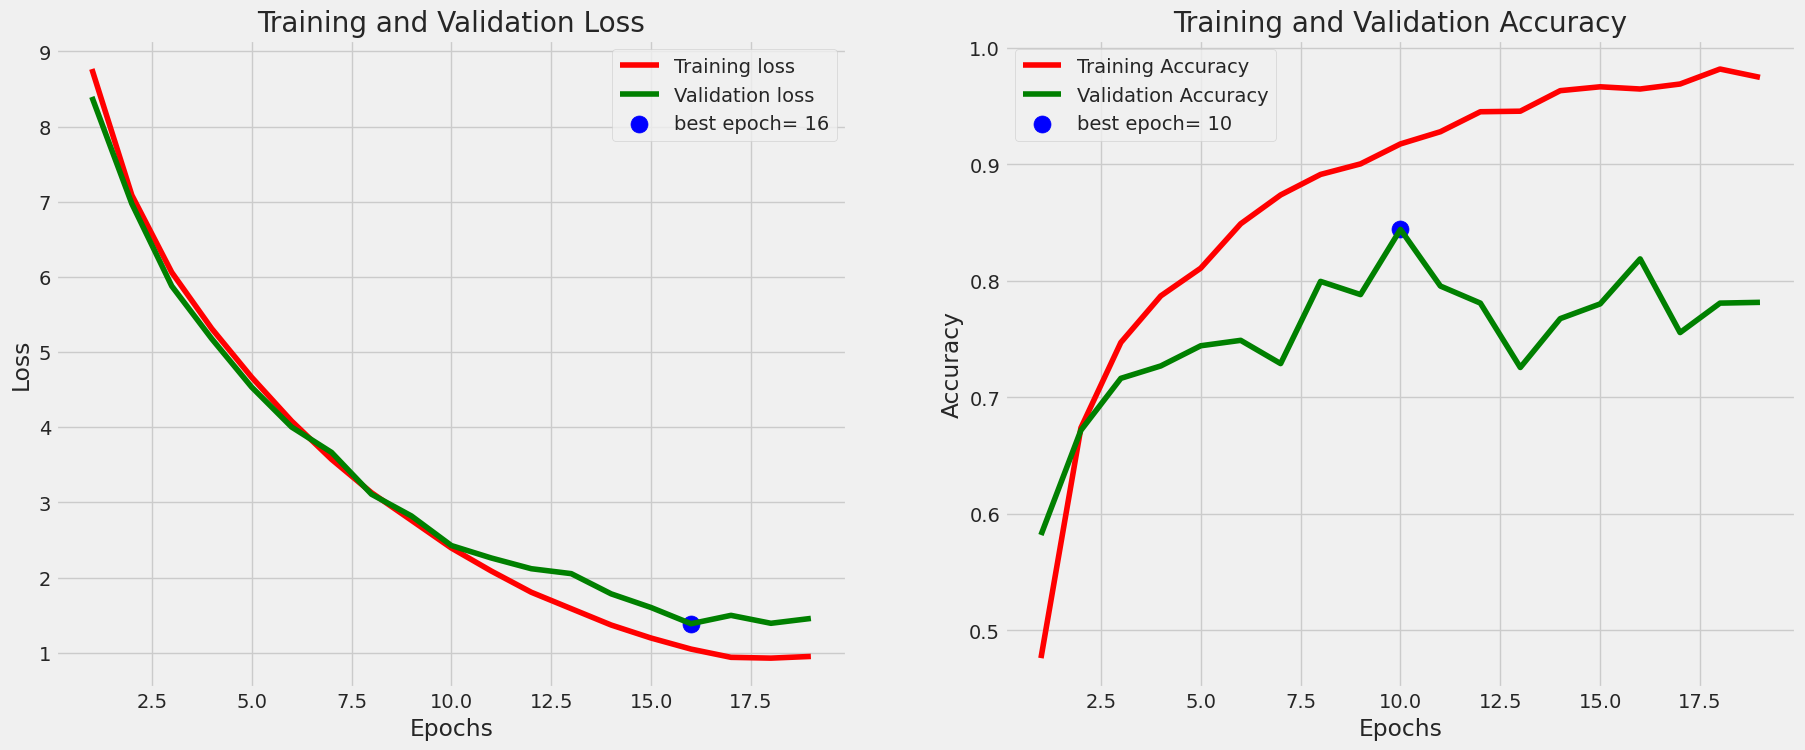
\includegraphics[width=1\textwidth]{./Graphics/training&validation_p2.png}
      \caption{Estadísticas de aprendizaje a lo largo del proceso de entrenamiento.\label{fig:training_validation_loss_p2}}
      \end{center}
		\end{figure}
  
La época con la mejor pérdida de validación y la mejor precisión de validación no coinciden, sugiere un trade-off entre la optimización de la pérdida y la maximización de la precisión. La volatilidad en la precisión de validación sugiere que el modelo puede beneficiarse de un ajuste en el tamaño del lote para suavizar las actualizaciones de los pesos y mejorar la estabilidad del modelo.

Dado lo anterior, se hizo una última iteración del modelo aumentando el volumen de muestras por clase a 500. Estos fueron los resultados. Se obtuvo una efectividad de aproximadamente 87\% (86.83\%).

\begin{figure}[ht]%
   \begin{center}
   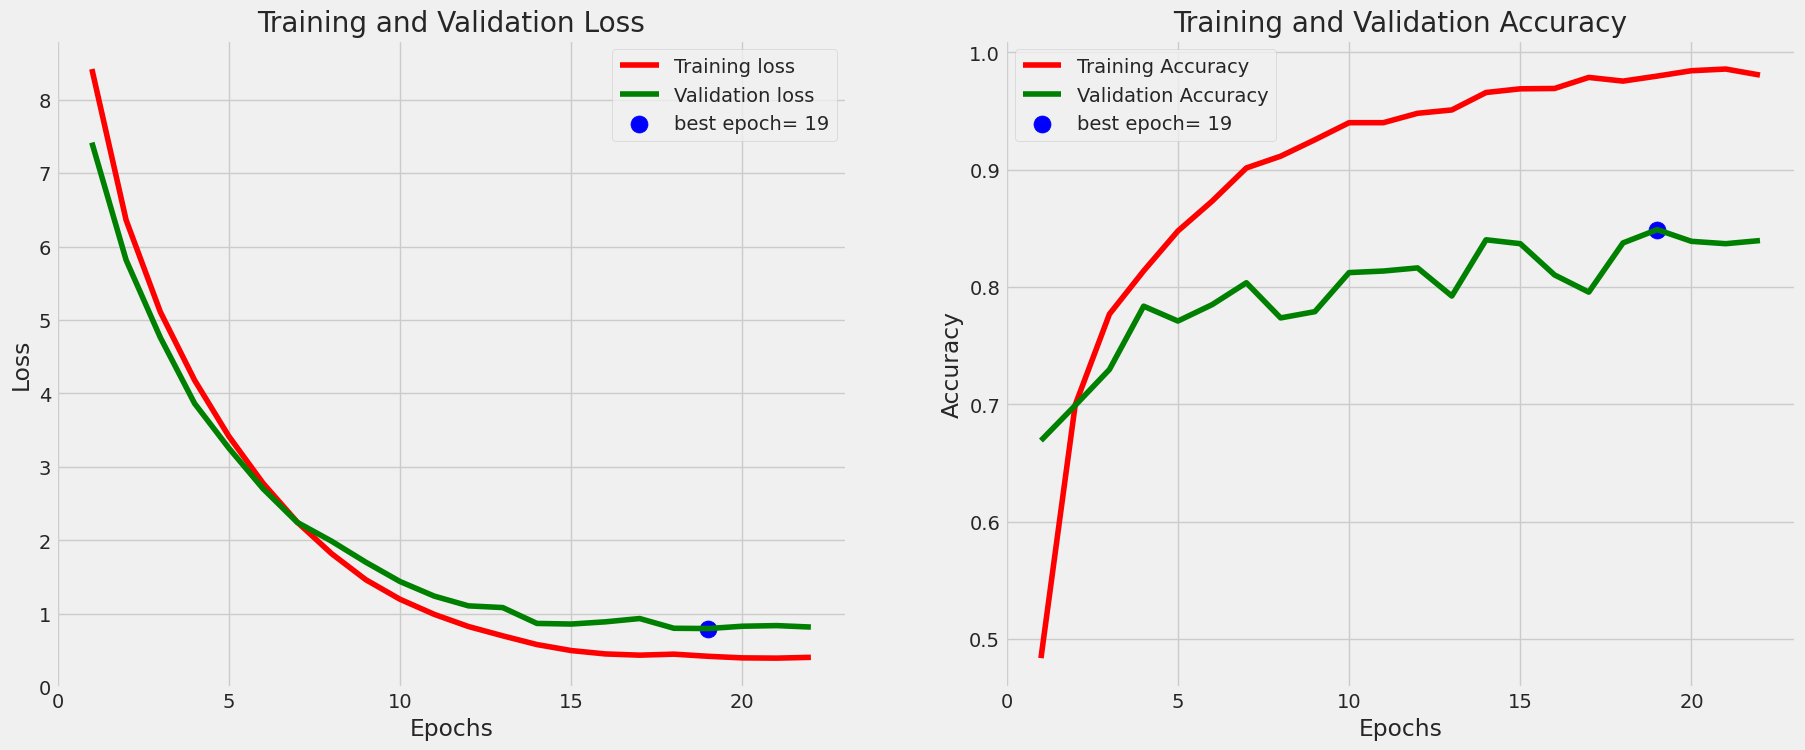
\includegraphics[width=1\textwidth]{./Graphics/training&validation_p3.png}
   \caption{Estadísticas de aprendizaje a lo largo del proceso de entrenamiento.\label{fig:training_validation_loss_p3}}
   \end{center}
   \end{figure}

La disminución continua en la pérdida de entrenamiento y la tendencia ascendente en la precisión de entrenamiento sugieren que el modelo está aprendiendo de manera efectiva y consistente. La pérdida de validación que converge con la de entrenamiento y la mejor época coincidente para pérdida y precisión de validación (época 19) indican que el modelo generaliza bien y no solo memoriza los datos de entrenamiento.

En el gráfico actual, hay una mejor alineación entre la pérdida de entrenamiento y validación y menos volatilidad en la precisión de validación, lo que indica un modelo más estable.

%-----------------------------------------------------------------------------------
	\subsection{Estadísticas de eficacia}\label{sub:accuracy_statistic_p2}
%-----------------------------------------------------------------------------------
    
\begin{figure}[ht]%
   \begin{center}
   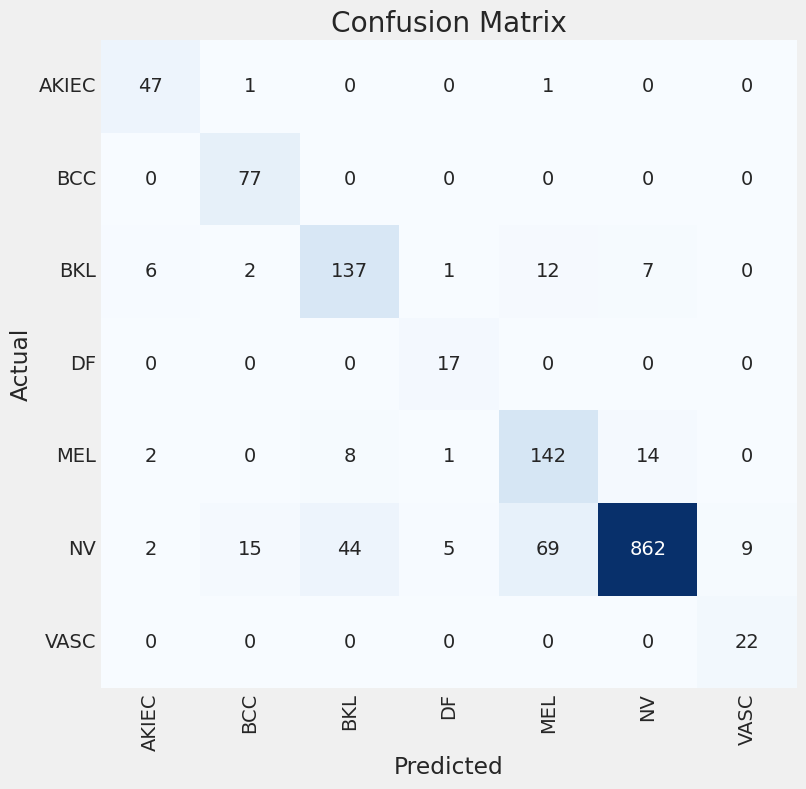
\includegraphics[width=1\textwidth]{./Graphics/confussionMatrix_p3.png}
   \caption{Estadísticas de eficacia del modelo al estimar los resultados en el conjunto de pruebas\label{fig:confussion_matrix_p3}}
   \end{center}
   \end{figure}

   \begin{figure}[ht]%
      \begin{center}
      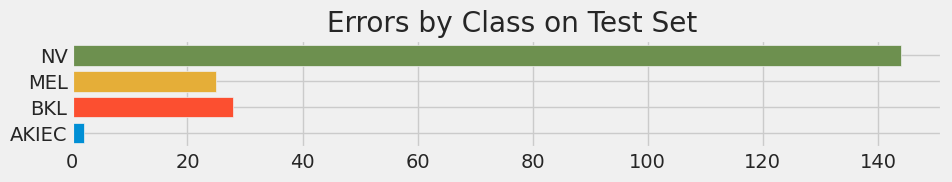
\includegraphics[width=1\textwidth]{./Graphics/errorByClass_p3.png}
      \caption{Gráfico de errores por clase en el conjunto de pruebas\label{fig:class_errors_p3}}
      \end{center}
      \end{figure}

NV muestra la mayoría de los errores, lo que puede deberse a una mayor prevalencia en el conjunto de datos.

Comparando ambos gráficos, podemos identificar áreas específicas donde el modelo necesita mejora. Por ejemplo, la clase 'NV', a pesar de tener muchas predicciones correctas, tiene un número relativamente alto de falsos positivos y falsos negativos, lo que sugiere que puede haber características de las imágenes 'NV' que se confunden con otras clases. En cambio, 'BCC' y 'DF' parecen estar bien diferenciados del resto. Esto puede informar estrategias futuras para mejorar la precisión del modelo, como la recolección de más datos o la implementación de técnicas de aprendizaje más avanzadas para clases específicas.